\chapter{Dataset and Data Representation}
\paragraph{Overview}
This chapter aims to be a description of the dataset structure the model is trained and evaluated with, as well as an overview of the processes that led to the creation of the dataset themselves.
In section~\ref{sec:Sources} a reference to the data sources is given, then the focus of section~\ref{sec:WAD} is on how data is natively encoded for the game engine in order to give some hints on what are the difficulties to face in converting to and from that format in an automatic way. Section~\ref{sec:TargetFormat} describes in detail what data is provided with the dataset, how levels are converted from the native format and what features are extracted in order to provide an input for the neural network. Lastly, section~\ref{sec:DatasetOrganization} gives an overview of how the data is provided and organized in the resulting dataset.
 
\section{Data Sources}
\label{sec:Sources}
\paragraph{Archive} All data used to train and validate the model comes from the \textit{Idgames Archive} founded in 1994 by Barry Bloom \cite{idarchivehistory} and mirrored on various FTP sources. The mirror we used for collecting levels is Doomworld.com \cite{url:doomworld}, which is one of the oldest and currently most active community about the DOOM video-game series \cite{wiki:doomworld}.
\paragraph{Level Selection} Idgames archive includes levels for multiple games such as DOOM, DOOM 2 or their various modifications. They are divided in hierarchical categories, which classify levels by game, game mode (multi-player "deathmatch" or single-player), and alphabetically.
Amongst all the categories we selected only those levels that belong to "DOOM" and "DOOM 2", excluding sub-categories named "deathmatch" and "Ports". This choice has been made in order to avoid mixing possibly different kinds of levels, since a level designed for a Single Player Mode could be structurally different from a level which is designed for multi-player games. Moreover the "Ports" category has been excluded because levels contained in it are intended to work with modifications of the game engine code, and it would have led to problems in managing every particular exceptional behaviour.

\paragraph{Source Data Organization} Levels in Idgames archive are stored in zip archives, including a "READ ME" text file containing author notes and the \gls{WAD} file that contains up to 32 levels. 
Each zip archive can be downloaded from the respective download page, which presents a variable quantity of information such as: author, a short description, screen shots, user reviews, number of views and downloads, etc.
The dataset we present in this work always keeps track of these information about each level for correct attribution. It also offers a "snapshot" of average user review score and the number of views and downloads, when available. It is worth noting that since Doomworld website recently switched to a different download system \cite{wiki:doomworld}, data may not always be accurate, especially that concerning download and view counts; they are still proposed as a starting point for further research. 
\section{Source Data Format: WAD Files}
\label{sec:WAD} 
\paragraph{Introduction} The Doom Game Engine \cite{doomengine} makes use of package files called "\glspl{WAD}" to store every game resource such as Levels, Textures, Sounds, etc. 
\gls{WAD} files have been designed in order to make the game more extendible and customizable, and opened the way for a considerably large amount of user-generated content. This section is not meant to be a complete description of how \glspl{WAD} files are structured, but only an overview of which aspects we considered for writing the software that generates the dataset from the \gls{WAD} files. Every information about \glspl{WAD} files has been taken from the \citetitle{doomspecs} \cite{doomspecs} and we refer to that document a deeper explanation on every aspect of the file format.
\subsection{Overview}
\paragraph{Type of WADs}
There are two types of \glspl{WAD}: the "IWAD", or "Internal WAD", and the "PWAD" or "Patch WAD". The original game files, called "DOOM.WAD" and "DOOM2.WAD", are of the "IWAD" type, as they contain every asset that is needed for the game to run. The \glspl{WAD} containing custom content or modifications to existing content are of the "PWAD" type. The content which is defined in a PWAD is added or replaced to the original IWAD when the \gls{WAD} is loaded. For example, if a PWAD defines the level "MAP01", which is already defined in "DOOM2.WAD", the PWAD level is loaded instead of the original one, while maintaining all the other content unaltered.
Since in our work we deal only with PWADs, we will generally refer to them simply as \glspl{WAD}.

\paragraph{Lumps} Every data inside a \gls{WAD} is stored as a record called \gls{lump}, which has a name up to 8 characters and a structure and size that is different depending on the lump type. Generally there are no restrictions on lump order with the exception of some of them, including those needed for defining a Level.

\paragraph{WAD Structure} Every \gls{WAD} file is divided in three sections: A header, a set of \glspl{lump} and a trailing Directory. The header holds the information about the WAD type, the number of \glspl{lump} and the location of the Directory, which is positioned after the last \gls{lump}. The directory contains one 12-bytes entry for each \glspl{lump} that specifies the \glspl{lump} location, size and name. Table~\ref{tab:WADStructure} reports a simplified description of a \gls{WAD} file.



\begin{table}[b]
	\centering
	\begin{tabularx}{\textwidth}{| c | c | c | c | X | }
		\hline
		Section Length (bytes) & Section Name & Field Size & Field Name & Description \\
		\hline
		   &   & 4 & Identification & ASCII string "PWAD" or "IWAD" \\ \cline{3-5}
		12 &     Header			  & 4 & Number of Lumps & The number of Lumps included in the WAD \\  \cline{3-5}
		&   						  & 4 & Table Offset & Integer pointer to the Dictionary \\ \cline{3-5}
		\hline
		Variable& Lumps & - & Lump Data & Lumps stored as a stream of Bytes \\
		\hline
		&                              & 4 & Lump Position & Integer holding a point to the lump's data \\ \cline{3-5}
		16 * Number of Lumps  & \multirow{3}{*}{}{Directory} & 4 & Lump Size & Size of the lump in bytes \\ \cline{3-5}
		&                              & 8 & Lump Name & Lump name in ASCII, up to 8 bytes long. Shorter names are null-padded \\ \cline{3-5}
		\hline
	\end{tabularx}
\caption{WAD File structure}
\label{tab:WADStructure}
\end{table}

\paragraph{Coordinate Units} \label{par:coords} The Doom game engine describes coordinates using integer values between -32768 and +32767, and it is proportional to one pixel of a texture. This unit is called "Map Unit" or "Doom Unit" in this work. Although there's not an unique real world interpretation of one Map Unit, we used an approximation for which each relevant map tile or image pixel is 32x32 MU large; this choice is motivated by the fact that the smallest radius of a functional object in DOOM is 16 MU. 

\newpage

\subsection{Doom Level Format}
\paragraph{Overview} Level data in a \gls{WAD} file follows a precise structure. In particular each level is composed of an ordered sequence of lumps that describes its structure:
	\begin{description}[wide=\parindent]
		\item[(NAME)]: Name of the level slot in DOOM or DOOM2 format.
		\item[THINGS] List of every game object ("\gls{thing}") that is placeable inside the level.
		\item[LINEDEFS] List of every line that connects two vertices.
		\item[SIDEDEFS] A list of structures describing the sides of every Linedef.
		\item[VERTEXES] Unordered list of vertices.
		\item[SEGS] A list of linedef segments that forms sub-sectors.
		\item[SSECTORS] A list of sub-sectors, which are convex shapes forming sectors.
		\item[NODES] A binary tree sorting sub-sectors for speeding up the rendering process.
		\item[SECTORS] A list of Sectors. A \gls{sector} is a closed area that has the same floor and ceiling height and textures.
		\item[REJECT] Optional lump that specifies which sectors are visible from the other. Used to optimize the AI routines.
		\item[BLOCKMAP] Pre-computed collision detection map. 
	\end{description}

\paragraph{Essential Subset and Optimizations} It is important to notice that although all the lumps above (with the exception of REJECT) are mandatory to build a playable level, some of them can be automatically generated from the remaining ones using external tools. In particular, an editor software or designer has to provide at least the lumps (name), THINGS, LINEDEFS, SIDEDEFS, VERTEXES and SECTORS. The lumps SEGS, SSECTORS, NODES, REJECT and BLOCKMAP serve the purpose of speeding-up the rendering process by avoiding runtime computation. In particular the Doom Engine uses a Binary Space Partitioning Algorithm \cite{Fuchs:1980:VSG:965105.807481} for pre-computing the Hidden Surface Determination (or occlusion culling), and it is usually done by an external tool. In this work we used the tool "\citetitle{bsp}" \cite{bsp} in the last stage of the pipeline, in order to produce playable DOOM levels from the network output. In the following paragraphs only the lump types that are not generated by the external tool are described.

\paragraph{(Name)} \label{slotname} The first lump of a level is its slot name. We indicate this lump between parenthesis because, differently from the other lumps, this one has no data associated. The Name field in the Directory is the slot name itself and the size is therefore zero. The level name descriptor has to match either \textit{ExMy} ("Episode x, Map y") or \textit{MAPzz} for DOOM or DOOM2 respectively, where x ranges from 1 to 4, y from 1 to 9 and zz from 1 to 32.


\paragraph{Things} A doom "\gls{thing}" is every object included in a level that is not a wall, pavement, or a door. A "Things" lump is a list of entries each one containing five integers specifying the \textit{position} (x,y) in \gls{MU}, the \textit{angle} the thing is facing, the \textit{Thing type} index, and a set of flags indicating in which difficulty level the thing is present and whether the thing is deaf, if it is an enemy.

\paragraph{Linedefs} A \gls{linedef} is any line that connects two vertices. Since DOOM maps are actually bi-dimensional, a single line is needed to define each wall or step. \glspl{linedef} do not necessarily have to match with visible entities, as each \gls{linedef} can also represent invisible boundaries or triggers, which can be thought as tripwires or switches that make something happen to a sector. If the \gls{linedef} acts as a trigger than it references another sector and has a type which defines what would happen to it when the \gls{linedef} is activated. For example, a door is implemented as a sector that raises up to the ceiling when a certain \gls{linedef} is triggered, but this behaviour is specified in the switch and not in the door as one might think. All the options are defined by a set of flags that specifies what kind of objects the \gls{linedef} blocks, if it's two sided or not, the trigger activation condition and so on.
Finally, each \gls{linedef} has to specify what "vertical plane" (or \gls{sidedef}) lies on its right and left side. Only the "left sidedef" field can be left empty, due to the way the sectors are represented.

\paragraph{Sidedefs} A \gls{sidedef} is a structure that contains the texture data for each linedef. It corresponds to the side of each wall and it's referenced by the linedefs. Other than the options for texture visualization, it also specifies the sector number that this plane is facing, implicitly defining the sector boundaries.

\paragraph{Vertexes}\footnote{Although the correct spelling should be "vertices", we keep the original version of the field name.} This is the simplest type of \gls{lump}, consisting in an unordered list of map coordinates in \gls{MU}. Each entry has an x and y position expressed in a 16-bit signed integer. \glspl{linedef} references the starting and ending vertex by reporting their index in this list.

\paragraph{Sectors} A sector is defined as any area that have constant floor and ceiling heights and textures. This definition highlights the fact that the doom engine is in fact a 2d engine, since it's not possible to define a sector above or below another one. A sector does not necessarily have to be closed nor a single connected polygon, but non-closed sectors can cause some issues during gameplay. The only constraint to define sectors comes from the fact that linedefs must have a right sidedef, but the left one is optional; the sectors are normally described as (a set of) positively oriented curves \cite{poly_orient}, with the exception of linedefs that are shared with another sector that may be reversed. The fields of a sector lump includes the floor and ceiling height, the name of the floor and ceiling texture, the light level, the "type" to controls some lighting effects and damaging floor, and the tag number that is referenced by the linedef triggers. Figure~\ref{fig:sectors} shows an example of a level with 3 sectors.


\begin{figure}
	\begin{center}
		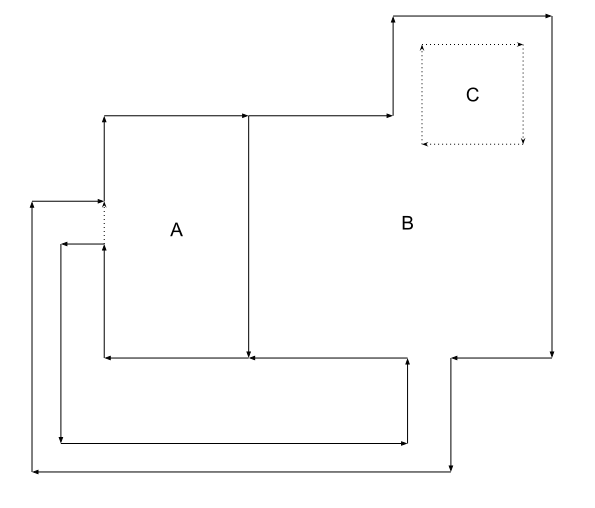
\includegraphics[width=0.8\linewidth]{linedefs_and_sectors}
	\end{center}
	
	\captionsetup{width=0.8\linewidth}
	\caption[A simple level showing sectors and linedefs]{A simple level showing three sectors A, B and C and the linedefs defining them, following the positive oriented curve constraint. Sector C can be viewed as a small platform inside the sector B. Solid arrows represent walls, while dashed lines represent invisible linedefs or changes in height between two sectors (steps). In this level, every solid arrow is a linedef that specifies only a right sidedef, with the exception of the one separating sectors A and B that has both a right and a left one.}
	\label{fig:sectors}
	\medskip
	
\end{figure}


\subsection{Conversion issues} 
Since 1994 many DOOM players started producing a large amount of levels and increasingly sophisticated editors came to light. This led to a notable variety in conventions, optimizations and use of bad practices that we tried to deal with in developing the Python module for reading and writing wad files. Some of these practices includes unnecessary lumps, random-data instead of null padding for names, and other inconsistencies or arbitrary conventions. 
However, we paid particular attention during the writing phase in order to precisely follow the specifications and avoid generating low quality WAD files as much as we could.
Some other difficulties came with the necessity to render wad files as images and vice-versa. The first one is that neither \glspl{linedef} nor vertices came in an any ordered format, along with the fact that sector vertices are not explicitly defined, but only referenced through the linedef/sidedef chain. This means that for finding a sector shape one has to find all sidedefs with the desired sector number, then find all the linedefs referencing those sidedefs and lastly retrieving the vertices, leading to an increase of complexity. Another problem was the fact that although sectors must be positively oriented curves, it is not mandatory to use the left sidedefs for adjacent sectors, leading to duplicated linedefs in the opposite direction. Even some optimizations such as sidedef compression may be possible, that is referencing the same sidedef wherever the same wall texture is used, adding complexity to the conversion script. Moreover, the concept of sector and the concept of room are not equivalent: even though a sector is defined as an area of constant height, this does not enforce to define a sector only where height changes, so the semantic of a sector actually depends on the designer and the editor used. 


\section{Target Data Format: Feature Maps and Vectors}
\label{sec:TargetFormat}
\paragraph{Introduction} This section provides a description of the data format as it is stored in the level dataset.
\subsection{Level Description and Motivation}
%TODO: Perché le immagini? Come mai divise così? Come mai l'encoding in questo modo?
\paragraph{}Levels are read as a structured object by a module we wrote for the purpose of providing developers and designers a programmatic way to access, analyse and edit DOOM WAD files, instead of using visual authoring software. This allows to automatise some tasks that would be very long to accomplish with standard editors or tools and also offers developers the possibility to write custom editor and scripts. \\*
In order to provide the most complete set of information possible every level is converted to a set of images, called \glspl{featuremap} in this work, a tiled representation in textual format that is an extension of the one taken from \cite{VGLC}, a graph representation and a set of textual and scalar features that contains both the \gls{WAD} meta-data and the level features and metrics calculated either on the WAD representation (sectors, subsectors, linedefs, etc), the \gls{featuremap} representation or the graph representation of the level. A detailed list and explanation of each feature is provided in section~\ref{features}. \\*
The choice of these representations have been made primarily for the need of having a data format that the generator model can work  on. In particular, convolutional neural netoworks are naturally designed to work well with bi-dimensional or tri-dimensional data such as (multi-channel) images, for this reason the image representation arose naturally. The text representation is provided mainly for consistency with the data format given in \cite{VGLC}, even if our representation uses two characters per tile instead of one. Finally, scalar and graph representation have been collected for the need of quantifying and summarising some properties and having a more abstract representation of a level, which can be very helpful in the case this data had to be used in other works.

\subsection{Feature Maps}
%TODO: Describe the maps and data encoding
\paragraph{} \glspl{featuremap} are a set of images each of them describing a different aspect of the level. In particular we used for each \gls{featuremap} a grayscale 8-bit image in which each pixel can assume values between 0 an 255. This allowed to obtain a good degree of precision while still maintaining a reasonable dataset size. \\*
Because of the motivations explained in section~\ref{par:coords}, each pixel in a \gls{featuremap} corresponds to a square of 32x32 \gls{MU}. 
In the following paragraph we will describe in detail each of them along with the data encoding.

\paragraph{\gls{floormap}} The \gls{floormap} is the most basic form of level representation, since it only represents which part of the space are occupied by the level and which are empty. This kind of map is often used in robotic mapping. \\*
This map also describes approximatively the level area that is possible to traverse, since in DOOM walls have no thickness. \\*
"Floor" pixels have value 255 (white) and "Empty" pixels have value 0 (black).

\paragraph{\gls{wallmap}} The \gls{wallmap} represent the impassable walls of the level. They are represented as a one-pixel-wide line and are obtained by directly drawing each \gls{linedef} with the impassable flag set on a black image. \\*
Pixel values are 0 for Empty area or floors and 255 for the walls.

\paragraph{\gls{heightmap}} The \gls{heightmap} is another common map used for visualizing the height of a certain surface. Since height level in DOOM levels are completely arbitrary and virtually unbounded, we normalize each level between its lowest and highest height, assigning the pixel value 0 for empty parts of the level and the remaining are calculated from the formula $ c_{h} = \lfloor h * \dfrac{255}{|H|} \rfloor $, where $ H $ is the ordered set of possible height values for the level and $ h \in \{1, 2, ..., |H| \} $ is the index of the height value in $ H $ for which we want to calculate the encoded colour. \\*
 For example if a level takes the height values $ H = \{ 0, 10, 15, 20 \} $ they will be encoded respectively as $ c_{h} = \{ 63, 127, 191, 255\} $ and 0 for the empty areas. Although this map loses the information about the differences between a height level and another, it has the advantage to represent "higher" and "lower" parts of the level without polarizing the entire map due to extreme levels: while the majority of the levels has a few changes that can be approximated as uniform (such as levels with stairs connecting a few rooms), other had some extreme changes in height but only for a small portion of the map (like a very high elevator leading to a small secret room) that led to scaling problems.
 
\paragraph{\gls{thingsmap}} The \gls{thingsmap} represent only data that is contained in the THINGS lump. It features a series of pixels placed at the thing coordinate, with a value that corresponds to a particular "thing". Pixel colours have been grouped by functional purposes so for example weapons occupies values that are close each other. This is for tolerating some output noise during generation without completely changing the functional aspect of an object as would have happened if we kept the original things encoding. Tables \ref{tab:thingsmap1}, \ref{tab:thingsmap2} and \ref{tab:thingsmap3} lists the complete encoding for the maps. Descriptions are taken from \cite{wiki:thingtypes}.

\begin{table}[b]
	\centering
	\begin{tabularx}{\textwidth}{| c | c | X | }
		\hline
		\textbf{Value} & \textbf{Functional Category} & \textbf{Thing Description} \\
		\hline
		0	& 	& Empty \\
		1	& other	& Boss Brain \\
		2	& other	& Deathmatch start \\
		3	& other	& Player 1 start \\
		4	& other	& Player 2 start \\
		5	& other	& Player 3 start \\
		6	& other	& Player 4 start \\
		7	& other	& Spawn shooter \\
		8	& other	& Spawn spot \\
		9	& other	& Teleport landing \\
		10	& keys	& Blue keycard \\
		11	& keys	& Blue skull key \\
		12	& keys	& Red keycard \\
		13	& keys	& Red skull key \\
		14	& keys	& Yellow keycard \\
		15	& keys	& Yellow skull key \\
		16	& decorations	& Bloody mess \\
		17	& decorations	& Bloody mess \\
		18	& decorations	& Candle \\
		19	& decorations	& Dead cacodemon \\
		20	& decorations	& Dead demon \\
		21	& decorations	& Dead former human \\
		22	& decorations	& Dead former sergeant \\
		23	& decorations	& Dead imp \\
		24	& decorations	& Dead lost soul (invisible) \\
		25	& decorations	& Dead player \\
		26	& decorations	& Hanging leg \\
		27	& decorations	& Hanging pair of legs \\
		28	& decorations	& Hanging victim, arms out \\
		29	& decorations	& Hanging victim, one-legged \\
		30	& decorations	& Hanging victim, twitching \\
		31	& decorations	& Pool of blood \\
		32	& decorations	& Pool of blood \\
		33	& decorations	& Pool of blood and flesh \\
		34	& decorations	& Pool of brains \\
						\hline
			\end{tabularx}
		\caption{ThingsMap Encoding (1 of 3)}
		\label{tab:thingsmap1}
		\end{table}
		
		\begin{table}[b]
			\centering
			\begin{tabularx}{\textwidth}{| c | c | X | }
				\hline
				\textbf{Value} & \textbf{Functional Category} & \textbf{Thing Description} \\
				\hline
		
		35	& obstacles	& Barrel \\
		36	& obstacles	& Burning barrel \\
		37	& obstacles	& Burnt tree \\
		38	& obstacles	& Candelabra \\
		39	& obstacles	& Evil eye \\
		40	& obstacles	& Five skulls "shish kebab" \\
		41	& obstacles	& Floating skull \\
		42	& obstacles	& Floor lamp \\
		43	& obstacles	& Hanging leg \\
		44	& obstacles	& Hanging pair of legs \\
		45	& obstacles	& Hanging torso, brain removed \\
		46	& obstacles	& Hanging torso, looking down \\
		47	& obstacles	& Hanging torso, looking up \\
		48	& obstacles	& Hanging torso, open skull \\
		49	& obstacles	& Hanging victim, arms out \\
		50	& obstacles	& Hanging victim, guts and brain removed \\
		51	& obstacles	& Hanging victim, guts removed \\
		52	& obstacles	& Hanging victim, one-legged \\
		53	& obstacles	& Hanging victim, twitching \\
		54	& obstacles	& Impaled human \\
		55	& obstacles	& Large brown tree \\
		56	& obstacles	& Pile of skulls and candles \\
		57	& obstacles	& Short blue firestick \\
		58	& obstacles	& Short green firestick \\
		59	& obstacles	& Short green pillar \\
		60	& obstacles	& Short green pillar with beating heart \\
		61	& obstacles	& Short red firestick \\
		62	& obstacles	& Short red pillar \\
		63	& obstacles	& Short red pillar with skull \\
		64	& obstacles	& Short techno floor lamp \\
		65	& obstacles	& Skull on a pole \\
		66	& obstacles	& Stalagmite \\
		67	& obstacles	& Tall blue firestick \\
		68	& obstacles	& Tall green firestick \\
		69	& obstacles	& Tall green pillar \\
		70	& obstacles	& Tall red firestick \\
		71	& obstacles	& Tall red pillar \\
		72	& obstacles	& Tall techno floor lamp \\
		73	& obstacles	& Tall techno pillar \\
		74	& obstacles	& Twitching impaled human \\
		
								\hline
	\end{tabularx}
\caption{ThingsMap Encoding (2 of 3)}
\label{tab:thingsmap2}
\end{table}

\begin{table}[b]
\centering
\begin{tabularx}{\textwidth}{| c | c | X | }
\hline
\textbf{Value} & \textbf{Functional Category} & \textbf{Thing Description} \\
\hline
		
		75	& monsters	& Arachnotron \\
		76	& monsters	& Arch-Vile \\
		77	& monsters	& Baron of Hell \\
		78	& monsters	& Cacodemon \\
		79	& monsters	& Chaingunner \\
		80	& monsters	& Commander Keen \\
		81	& monsters	& Cyberdemon \\
		82	& monsters	& Demon \\
		83	& monsters	& Former Human Trooper \\
		84	& monsters	& Former Human Sergeant \\
		85	& monsters	& Hell Knight \\
		86	& monsters	& Imp \\
		87	& monsters	& Lost Soul \\
		88	& monsters	& Mancubus \\
		89	& monsters	& Pain Elemental \\
		90	& monsters	& Revenant \\
		91	& monsters	& Spectre \\
		92	& monsters	& Spider Mastermind \\
		93	& monsters	& Wolfenstein SS \\
		94	& ammunitions	& Ammo clip \\
		95	& ammunitions	& Box of ammo \\
		96	& ammunitions	& Box of rockets \\
		97	& ammunitions	& Box of shells \\
		98	& ammunitions	& Cell charge \\
		99	& ammunitions	& Cell charge pack \\
		100	& ammunitions	& Rocket \\
		101	& ammunitions	& Shotgun shells \\
		102	& weapons	& BFG 9000 \\
		103	& weapons	& Chaingun \\
		104	& weapons	& Chainsaw \\
		105	& weapons	& Plasma rifle \\
		106	& weapons	& Rocket launcher \\
		107	& weapons	& Shotgun \\
		108	& weapons	& Super shotgun \\
		109	& powerups	& Backpack \\
		110	& powerups	& Blue armor \\
		111	& powerups	& Green armor \\
		112	& powerups	& Medikit \\
		113	& powerups	& Radiation suit \\
		114	& powerups	& Stimpack \\
		115	& artifacts	& Berserk \\
		116	& artifacts	& Computer map \\
		117	& artifacts	& Health potion \\
		118	& artifacts	& Invisibility \\
		119	& artifacts	& Invulnerability \\
		120	& artifacts	& Light amplification visor \\
		121	& artifacts	& Megasphere \\
		122	& artifacts	& Soul sphere \\
		123	& artifacts	& Spiritual armor  \\
		\hline
	\end{tabularx}
	\caption{ThingsMap Encoding (3 of 3)}
	\label{tab:thingsmap3}
\end{table}

\paragraph{\gls{triggermap}} The \gls{triggermap} is used for representing linedef triggers and the sectors which activates. Due to the vast amount of cases the doom engine can handle, only a few types of triggers have been considered. The mapping works by assigning an integer $ i \le 32 $ to every trigger object, and subdividing triggers types in 5 groups: local doors (the ones that are activable only if the players directly interact with them), remote doors, lifts, switches and teleports. Local doors can be normal or require a key of a certain colour in order to open, but they are not indexed by the trigger index since they don't require to be linked to other linedefs in order to be opened. Table~\ref{tab:triggermap} describes the encoding for each possible item $ i $.

\begin{table}
\begin{tabularx}{\textwidth}{| c | c | X | }
	\hline
	\textbf{Value} & \textbf{Functional Category} & \textbf{Thing Description} \\
	\hline
	0 &	None &	Empty \\
	10 &	local doors	 & Blue key local door \\
	12 &	local doors & Red key local door \\
	14 &	local doors	 & Yellow key local door \\
	16 &	local doors & Local door \\
	32+i &	remote doors &	Remote door with tag i \\
	64+i &	lifts &	Lift with tag i \\
	128+i &	switch &	Linedef that activates the i tag \\
	192+i &	teleports &	teleport to sector i \\
	255 &	exit &	Level Exit \\
	\hline
\end{tabularx}
\caption[TriggerMap Encoding]{TriggerMap Encoding: Each item i is connected to one or more objects. For example: switch (128+1) will open the door (32+1), raise the lift (64+1), etc.}
\label{tab:triggermap}
\end{table}

\paragraph{\gls{roommap}} The \gls{roommap} represent an enumeration of the rooms obtained with an algorithm that is very similar to the morphological approach used in \citetitle{7487234}\cite{7487234}: An euclidean distance transform \cite{edt} is first applied to the \gls{floormap} obtaining a map that we call \"Distance Map\" or \"DistMap\", then the local maxima are found \cite{localmax} such that each maximum has a minimum distance of 3 from the closest one, resulting in the room center coordinates that are used as markers for a Watershed segementation \cite{watershed} using the negative distance map as basin. This results in a room segmentation that is good enough for descriptive purposes while maintaining good performances.

\subsection{Graph Representation}
Another way to represent the level is by using a graph. In particular, this graph is a region adjacency graph \cite{Trémeau00regionsadjacency} built upon the \gls{roommap}, where the nodes represent the rooms and the edges are the boundaries they have in common. This graph is built primarily for computing some features about the level and for exploiting its convenient representation of the rooms during the WAD Writing phase: this graph can be annotated with the coordinates of walls belonging to each room, and this information can be used to build a level room-by-room, with the assumption that a room could approximate a sector.


\subsection{Text Representation}
\label{textrep}
A text representation is also available, following the work of \citeauthor{VGLC} in \cite{VGLC}. In particular the representation has been extended from one character per tile/pixel to two characters. This way it has been possible to add the information about the sector tag and the damaging floor. This representation is not currently used by our work but provided for consistence with previous works. Table \ref{tab:textmap} reports all the character used for this encoding.


\begin{table}
	\begin{tabularx}{\textwidth}{| c | l | c | X | }
		\hline
		\textbf{1st character} & \textbf{Description} & \textbf{2nd Character} & \textbf{Description} \\
		\hline
		"-" &	["empty","out of bounds"] &	"-" [ascii(45)] &	Empty, no tag \\
		"X" &	["solid","wall"] &	"." [ascii(46)] &	Tag 1 \\
		"." &	["floor","walkable"] &	"/" [ascii(47)] &	Tag 2 \\
		"," &	["floor","walkable","stairs"] &	"0" [ascii(48)] &	Tag 3 \\
		"E" &	["enemy","walkable"] &	... &	... \\
		"W" &	["weapon","walkable"] &	"m" [ascii(109)] &	Tag 64 \\
		"A" &	["ammo","walkable"] &	"\textasciitilde" [ascii(126)] &	Damaging floor \\
		"H" &	["health","armor","walkable"]	 &	 & \\
		"B" &	["explosive barrel","walkable"]	 &	 & \\
		"K" &	["key","walkable"]		 & & \\
		"\textless" &	["start","walkable"]		 & & \\
		"T" &	["teleport","walkable","destination"]		 & & \\
		":" &	["decorative","walkable"]		 & & \\
		"L" &	["door","locked"]		 & & \\
		"t" &	["teleport","source","activatable"]	 &	 & \\
		"+" &	["door","walkable","activatable"]		 & & \\
		"\textgreater" &	["exit","activatable"]		 & & \\
		\hline
	\end{tabularx}
	\caption[Textual Representation Encoding]{Extended Textual Representation Encoding: A second character has been added to the one used by \citetitle{VGLC}: Each tile is expressed by two characters "XY" where X is the type of object and Y is the tag of the tile.
		Every tile that has a tag number, activates (or is activated by) the object(s) with the same tag number. 
		So, e.g. "t/" is a teleport that leads to "T/" and "X." is a switch that activates the door "+." and possibly a floor ".."}
	\label{tab:textmap}
\end{table}


	

\subsection{Scalar Features}
\label{features}
Each level is annotated with 176 numerical and textual features which are divided in four categories:
\begin{enumerate}
	\item \textbf{IDGames Archive Metadata} Contain information collected from the database when levels have been downloaded. This information contains the author, the descriptions, download urls, level title, etc. Since a WAD file can contain up to 32 levels, this information is replicated for each level found in the WAD file. \\*
	 Listed in table~\ref{tab:featureidgames}
	\item \textbf{WAD-extracted features:} This features are low-level features collected directly when processing the WAD file and include the number of lines, things, sectors, vertices, the maximum and minimum coordinates, the level size in \gls{MU} etc. \\* Listed in table~\ref{tab:featuresWAD}
	\item \textbf{PNG-extracted features} These features are computed starting from the \gls{floormap} using an Image processing library for calculating morphological properties. Each feature is calculated both directly over the whole level and as simple statistics computed over its "floors" taken singularly. A "Floor" is intended as a part of level which is not connected to the rest of the level, thus is reachable only by means of a teleporter. \\*
	Listed in tables~\ref{tab:featuresPNG1}, \ref{tab:featuresPNG2}
	\item \textbf{Graph Features} Features computed on the room graph, inspired by the work of \citeauthor{Amigoni} in \cite{Amigoni}. They are used to provide a higher level representation of the level and an indicative distribution of the different room types. \\*
	Listed in table~\ref{tab:featuresgraph}
\end{enumerate}

\begin{table}
	\begin{tabularx}{\textwidth}{| l | X | c |}
		\hline
		\textbf{Feature Name} & \textbf{Description} & \textbf{Type} \\
		\hline
		author	&	Level Author	&	string\\
		description	&	Natural language level information	&	string\\
		credits	&	Natural language level information	&	string\\
		base	&	Natural language level information	&	string\\
		editor\textunderscore used	&	Natural language level information	&	string\\
		bugs	&	Natural language level information	&	string\\
		build\textunderscore time	&	Natural language level information	&	string\\
		rating\textunderscore value	&	doomworld.com level rating value	&	float\\
		rating\textunderscore count	&	doomworld.com vote count	&	int\\
		page\textunderscore visits	&	doomworld.com page visits	&	int\\
		downloads	&	doomworld.com download count	&	int\\
		creation\textunderscore date	&	Natural language level information	&	string\\
		file\textunderscore url	&	Download page url	&	string\\
		game	&	Doom or DoomII	&	string\\
		category	&	doomworld.com category (eg. a-z)	&	string\\
		title	&	Full level name	&	string\\
		name	&	level .zip filename	&	string\\
		path	&	relative path to wad file	&	string\\
		\hline
		
	\end{tabularx}
	\caption[ Features: IDArchive Metadata ]{ Features: IDArchive Metadata }
	\label{tab:featureidgames}
\end{table}	


\begin{table}
	\begin{tabularx}{\textwidth}{| l | X | c |}
		\hline
		\textbf{Feature Name} & \textbf{Description} & \textbf{Type} \\
		\hline
		number\textunderscore of\textunderscore lines	&	absolute number of lines in the level 	&	int \\ \hline
		number\textunderscore of\textunderscore things	&	absolute number of objects in the level	&	int \\ \hline
		number\textunderscore of\textunderscore sectors	&	absolute number of sectors (zones with same height) in the level	&	int \\ \hline
		number\textunderscore of\textunderscore subsectors	&	absolute number of subsector (convex subshapes of sectors) in the level	&	int \\ \hline
		number\textunderscore of\textunderscore vertices	&	absolute number of vertices in the level	&	int \\ \hline
		x\textunderscore max	&	maximum x coordinate	&	int \\ \hline
		y\textunderscore max	&	maximum y coordinate	&	int \\ \hline
		x\textunderscore min	&	minimum x coordinate	&	int \\ \hline
		y\textunderscore min	&	minimum y coordinate	&	int \\ \hline
		height	&	level original height in DoomUnits	&	int \\ \hline
		width	&	level original width in DoomUnits	&	int \\ \hline
		floor\textunderscore height\textunderscore [max\textbar min\textbar avg]	&	[max\textbar min\textbar avg] height for the floor	&	float \\ \hline
		ceiling\textunderscore height\textunderscore [max\textbar min\textbar avg]	&	[max\textbar min\textbar avg] height for the ceiling	&	float \\ \hline
		room\textunderscore height\textunderscore [max\textbar min\textbar avg]	&	[max\textbar min\textbar avg] difference between ceiling and floor height	&	float \\ \hline
		sector\textunderscore area\textunderscore [max\textbar min\textbar avg]	&	[max\textbar min\textbar avg] area of sectors in squadred doom map units	&	float \\ \hline
		lines\textunderscore per\textunderscore sector[max\textbar min\textbar avg]	&	[max\textbar min\textbar avg] count of sector sides	&	float \\ \hline
		aspect\textunderscore ratio	&	Ratio between the longest and the shortest dimension, since a rotation of 90° of the level does not alter playability	&	float \\ \hline
		walkable\textunderscore area	&	Number of pixels the player can walk on (nonempty\textunderscore size - walls)	&	int \\ \hline
		walkable\textunderscore percentage	&	Percentage of the level that is walkable	&	float \\ \hline
		number\textunderscore of\textunderscore \textless things\textunderscore type \textgreater	&	Total number of  \textless things\textunderscore type\textgreater in the level. \textless things\textunderscore type\textgreater: \{ artifacts, powerups, weapons, ammunitions, keys,monsters , obstacles, decorations \}	&	int \\ \hline
		\textless things\textunderscore type\textgreater\textunderscore per\textunderscore walkable\textunderscore area	&	Number of \textless things\textunderscore type\textgreater divided the walkable area in DMU. &	float \\ \hline
		start\textunderscore location\textunderscore [x\textbar y]\textunderscore px	&	[x\textbar y] coordinate (in pixels, dataset format) of the start location.	&	int \\ \hline
		slot	&	Name of the map slot. e.g "E1M1" or "MAP01"	&	string \\
		\hline
\end{tabularx}
\caption[ Features: WAD-extracted ]{ WAD-extracted features }
\label{tab:featuresWAD}
\end{table}	


\begin{table}
	\begin{tabularx}{\textwidth}{| l | X | c |}
		\hline
		\textbf{Feature Name} & \textbf{Description} & \textbf{Type} \\
		\hline
		floors	&	Number of non-connected sectors (only reachable by a teleport) of the level	&	int \\ \hline
		level\textunderscore area	&	Number of pixels composing the level	&	int \\ \hline
		floors\textunderscore area\textunderscore [mean\textbar min\textbar max\textbar std]	&	[mean\textbar min\textbar max\textbar std] number of pixels composing each floor	&	float \\ \hline
		level\textunderscore bbox\textunderscore area	&	Number of pixels of bounding box sorrounding the level	&	int \\ \hline
		level\textunderscore convex\textunderscore area 	&	Number of pixels of convex hull for the whole level	&	int \\ \hline
		floors\textunderscore convex\textunderscore area\textunderscore [mean\textbar min\textbar max\textbar std]	&	[mean\textbar min\textbar max\textbar std] Number of pixels of convex hull for each floor	&	float \textbar  int \\ \hline
		level\textunderscore eccentricity 	&	Eccentricity of the ellipse that has the same second-moments as the level. 	&	float \\ \hline
		floors\textunderscore eccentricity\textunderscore [mean\textbar min\textbar max\textbar std]	&	Eccentricity of the ellipse that has the same second-moments as each floor	&	float \\ \hline
		level\textunderscore equivalent\textunderscore diameter 	&	The diameter of a circle with the same area as the level	&	float \\ \hline
		floors\textunderscore equivalent\textunderscore diameter\textunderscore [mean\textbar min\textbar max\textbar std] 	&  [mean\textbar min\textbar max\textbar std] equivalent diameter calculated over the floors of the level	&	float \\ \hline
		level\textunderscore euler\textunderscore number 	&	Euler characteristic of the level. Computed as number of objects (= 1) subtracted by number of holes (8-connectivity).	&	int \\ \hline
		floors\textunderscore euler\textunderscore number\textunderscore [mean\textbar min\textbar max\textbar std] 	&	[mean\textbar min\textbar max\textbar std] euler number over the floors of this level	&	float\\
				\hline
	\end{tabularx}
\caption[ Features: PNG-extracted (1 of 2) ]{ PNG-extracted features (1 of 2) }
\label{tab:featuresPNG1}
\end{table}			

\begin{table}
	\begin{tabularx}{\textwidth}{| l | X | c |}
		\hline
		\textbf{Feature Name} & \textbf{Description} & \textbf{Type} \\
		\hline
		
		level\textunderscore extent 	&	Ratio of pixels in the level to pixels in the total bounding box. Non-empty size of the level.	&	float \\ \hline
		floors\textunderscore extent\textunderscore [mean\textbar min\textbar max\textbar std] 	&	[mean\textbar min\textbar max\textbar std] extent over the floors of the level	&	float \\ \hline
		level\textunderscore filled\textunderscore area 	&	Number of pixels of the level, obtained by filling the holes	&	int \\ \hline
		floors\textunderscore filled\textunderscore [mean\textbar min\textbar max\textbar std]\textunderscore mean 	&	[mean\textbar min\textbar max\textbar std] filled area over the floors of the level	&	float \\ \hline
		level\textunderscore major\textunderscore axis\textunderscore length 	&	The length of the major axis of the ellipse that has the same normalized second central moments as the level.	&	float \\ \hline
		floors\textunderscore major\textunderscore axis\textunderscore length\textunderscore [mean\textbar min\textbar max\textbar std]	&	[mean\textbar min\textbar max\textbar std] major axis length over the floors of the level	&	float \\ \hline
		level\textunderscore minor\textunderscore axis\textunderscore length 	&	The length of the minor axis of the ellipse that has the same normalized second central moments as the level	&	float \\ \hline
		floors\textunderscore minor\textunderscore axis\textunderscore length\textunderscore [mean\textbar min\textbar max\textbar std]	&	[mean\textbar min\textbar max\textbar std] minor axis length over the floors of the level	&	float \\ \hline
		level\textunderscore orientation 	&	Angle between the X-axis and the major axis of the ellipse that has the same second-moments as the level. Ranging from -pi/2 to pi/2 in counter-clockwise direction.	&	float \\ \hline
		floors\textunderscore orientation\textunderscore [mean\textbar min\textbar max\textbar std] 	&	[mean\textbar min\textbar max\textbar std] orientation over the floors of the level	&	float \\ \hline
		level\textunderscore perimeter 	&	Perimeter the level which approximates the contour as a line through the centers of border pixels using a 4-connectivity.	&	float \\ \hline
		floors\textunderscore perimeter\textunderscore [mean\textbar min\textbar max\textbar std] 	&	[mean\textbar min\textbar max\textbar std] perimeter over the floors of the level	&	float \\ \hline
		level\textunderscore solidity 	&	Ratio of pixels in the level to pixels of the convex hull image.	&	float \\ \hline
		floors\textunderscore solidity\textunderscore [mean\textbar min\textbar max\textbar std] 	&	[mean\textbar min\textbar max\textbar std] solidity over the floors of the level	&	float \\ \hline
		level\textunderscore hu\textunderscore moment\textunderscore [0 ... 6] 	&	Hu moments (translation, scale and rotation invariant).	&	float \\ \hline
		level\textunderscore centroid\textunderscore x 	&	Centroid coordinate x	&	float \\ \hline
		level\textunderscore centroid\textunderscore y 	&	Centroid coordinate y	&	float\\
		\hline
	\end{tabularx}
	\caption[ Features: PNG-extracted (2 of 2) ]{ PNG-extracted features (2 of 2) }
	\label{tab:featuresPNG2}
\end{table}			


\begin{table}
	\begin{tabularx}{\textwidth}{| l | X | c |}
		\hline
		Feature Name & Description & Type \\
		\hline
		art-points	&	Number of articulation points in the room adjacency graph. An articulation point is a node which removal would result in a bipartite graph	&	int\\
		assortativity-mean	&	Mean assortativity. Assortativity is the tendency of one node to be connected with similar nodes.	&	float\\
		betw-cen-[min \textbar  max \textbar  mean \textbar  var]	&	Node centrality statistic calculated with the betweenness method	&	float\\
		betw-cen-[skew \textbar  kurt ]	&	Node centrality statistic calculated with the betweenness method	&	float\\
		betw-cen-[Q1 \textbar  Q2 \textbar  Q3]	&	Node centrality statistic calculated with the betweenness method	&	float\\
		closn-cen-[min \textbar  max \textbar  mean \textbar  var]	&	Node centrality statistic calculated with the Closeness method	&	float\\
		closn-cen-[skew \textbar  kurt]	&	Node centrality statistic calculated with the Closeness method	&	float\\
		closn-cen-[Q1 \textbar  Q2 \textbar  Q3]	&	Node centrality statistic calculated with the Closeness method	&	float\\
		distmap-[min \textbar  max \textbar  mean ]	&	Maximum value in the distance map, i.e. the size of the largest room. Background is ignored from computation.	&	float\\
		distmap-[var \textbar  skew \textbar  kurt]	&	Mean value for the distance map, i.e. the mean room size.  Background is ignored from computation.	&	float\\
		distmap-[Q1 \textbar  Q2 \textbar  Q3]	&	Skewness of the distnace distribuiton  Background is ignored from computation.	&	float\\
		\hline
	\end{tabularx}
	\caption[ Features: Graph ]{ Graph features }
	\label{tab:featuresgraph}
\end{table}	


\section{Dataset Organization}
\label{sec:DatasetOrganization}
\subsection{Overview}
This section will describe how the dataset is stored and how it can be used for future works. \\* 
Since the dataset has been created primarily for instructing a neural network to generate new levels, the choices in data formats and data representation have been made to increase re-usability and flexibility in data manipulation. In particular the full dataset is stored first as a set of files indexed by a JSON dictionary, but for various reason that will be explained more in depth in  chapter~\ref{sec:InputSelection} in our work we only used a subset of levels stored as a separated archive.
% Full dataset ha dimensioni reali, i tfrecords sono compressi e filtrati, etc.
\subsection{Full Dataset and Filtered Dataset}
In order to keep as much information as possible from the collected levels, we structured the representation of the DOOMDataset as follow:
\begin{itemize}
	\item  A \textbf{Full Dataset} containing all the levels we collected from the Idgames Archive.
	\item A set of \textbf{Filtered Datasets} containing a subset of levels that satisfy certain constraints and which are ready to use with TensorFlow \cite{tensorflow2015-whitepaper}.
\end{itemize}
\paragraph{Full Dataset} 
 The full dataset is kept as much portable as possible, in the sense that it shouldn't need particular technologies to be accessed except the capability of parsing JSON files and NetworkX \cite{networkx} for analysing the graph structure. \\*
 It is composed of about 9172 levels organized as a directory structure, while the maps are of different sizes given by the rescaling of the levels in \gls{MU} to tile/pixel format.\\*
 The folder is structured as follow:
 \begin{itemize}
 	\item \textbf{dataset.json} Contains all the scalar and textual information explained in section~\ref{features} and the relative paths to the files in sub-directories. Acts as a level database. 
 	\item \textbf{Original:} Contains all the WAD files as extracted by the archives downloaded from the IDGames Archive.
 	\item \textbf{Processed:} Contains the \glspl{featuremap}, the graph representation, the text representation and the relative set of features. \\*
 	Data in this folder is named as:
 	\begin{itemize}
		\item [\textbf{zipname\textunderscore WADNAME\textunderscore SLOT.json}] Is a json file containing all the features (\ref{features}) for the level.
		\item [\textbf{zipname\textunderscore WADNAME\textunderscore SLOT.networkx}] Is a gpickle compressed file containing the NetworkX graph for the level.
		\item [\textbf{zipname\textunderscore WADNAME\textunderscore SLOT.txt}] Is the Text Representation (\ref{textrep}) of the level
		\item [\textbf{zipname\textunderscore WADNAME\textunderscore SLOT\textunderscore mapname.txt}] Is the set of \glspl{featuremap} in PNG 8-bit greyscale format. 
 	\end{itemize}
 	Where zipname, wadname, mapname indicate the name of the zip archive the \gls{WAD} was stored in, the wad file itself and the \gls{featuremap} respectively, while SLOT indicates the level slot name in DOOM format (see section \ref{slotname}, "NAME" lump).
 	The choice of keeping features both in the JSON database and in separated files comes from the need of recomputing the features in an easy way (for example for adding features) and for providing the possibility to manually pick or inspect level properties without the need of accessing a long json file. This, however, comes at the cost of some data redundancy. 
 \end{itemize}


 
 \paragraph{Filtered Dataset} Due to technological limitations given by the machines used for training and other reasons explained in chapter~\ref{sec:InputSelection}, data is filtered according to some criteria in order to make them uniform in term of \gls{featuremap} size and removing some level exposing extreme values of the features. Filtered dataset is stored as a set of files described as follor:
 	\begin{itemize}
		\item \textbf{DATASETNAME-train.TFRecord} Dataset used for training the network using the TFRecord data format, which is a binary data format proposed by TensorFlow for improving data ingestion performances. 
		\item \textbf{DATASETNAME-validation.TFRecord}  Dataset used for model validation stored in TFRecord data format.
		\item \textbf{DATASETNAME.meta} Metadata and statistics about the dataset contained in train and validation datasets, in JSON format. Since the TFRecord format currently does not natively hold any information about the data contained in its records, it is useful to save data such as the item count, data structure and statistics about the dataset in a separate file, for easing the process of data normalization and other kind of operations.
 	\end{itemize}
 
 In our GitHub Repository \cite{gitrepo} it is possible to find the files relative to two different data subset:
 \begin{itemize}
 	\item \textbf{128-many-floors} Dataset of images up to 128x128 pixels (smaller levels are centered and padded) which have any number of floors, consisting of 1933 levels in training set and 829 in validation set. 
 	\item \textbf{128-one-floor} Dataset of images up to 128x128 pixels (smaller levels are centered and padded) which have just one floor, consisting of 1104 levels in training set and 474 in validation set.
 	
 \end{itemize}
	\paragraph{Provided Methods} The code repository \cite{gitrepo} hosts a Python module that provides all the necessary methods to inspect and analyse and rebuild both the full dataset and the filtered dataset. Further information is provided in the code documentation as it goes beyond the scope of this chapter.
	
\subsection{Level Size Statistics}
In this section we analyse how the level dimensions in \gls{MU} are distributed in the Full Dataset. Table \ref{tab:sizepercentiles} reports the percentile distributions for both the level height and the level width in Map units and Pixels. This distribution highlights how the choice of scaling 32 Doom units to a single pixel in order to avoid loosing functional information about the levels also leads to reasonable image sizes, since more than 80 percent of the levels are representable in with an image of 256 pixels in both height and width. Joint distribution of width and height is represented in figure~\ref{fig:sizedistribution}

\begin{table}[h!]
	\begin{tabularx}{\textwidth}{| X | c | c | c | c |}
		\cline{0-4}
		\textbf{Percentile} &  \textbf{Width in DU} & \textbf{Width in pixels} &\textbf{ Height in DU} & \textbf{Height in pixels} \\
		\cline{0-4}
		10th & 2305 & 72 & 2065 & 64 \\  
		20th & 3017 & 94 & 2657 & 83 \\  
		30th & 3633 & 113 & 3137 & 98 \\  
		40th & 4161 & 130 & 3606 & 112 \\  
		50th & 4737 & 148 & 4101 & 128 \\  
		60th & 5393 & 168 & 4657 & 145 \\  
		70th & 6177 & 193 & 5313 & 166 \\  
		80th & 7212 & 225 & 6209 & 194 \\  
		90th & 9040 & 282 & 7809 & 244 \\
		100th & 31233 & 976 & 32743 & 1023 \\   
		\cline{0-4}
\end{tabularx}
\caption[ Percentiles of level width and height distributions ]{  Percentiles of level width and height distributions in both Map Units and Pixels }
\label{tab:sizepercentiles}
\end{table}	


\begin{figure}[h!]
	\begin{center}
		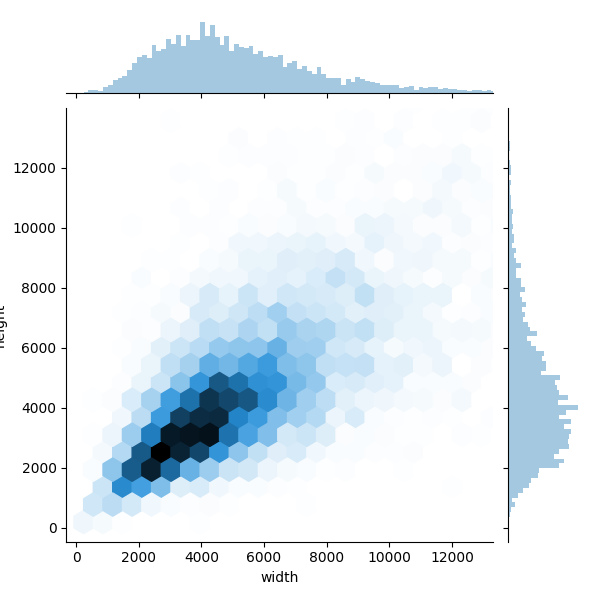
\includegraphics[width=0.8\linewidth]{dataset_dimension_distribution}
	\end{center}
	
	\captionsetup{width=0.8\linewidth}
	\caption[DoomDataset Size distribution]{Joint distribution for the features "width" (on the x axis) and "height" (on the y axis) expressed in \gls{MU} for the level contained in the full dataset. It is possible to notice how the size of the majority of the levels are below 7000 Map Units   }
	\label{fig:sizedistribution}
	\medskip
	
\end{figure}

\newpage
\section{Summary}
In this chapter we proposed a setting for describing the structure and the features of DOOM levels, analysing the WAD file format and exploiting its properties to extract useful data. Inspired by the work of \citeauthor{VGLC} in \citetitle{VGLC} we produced a dataset of more than 9000 DOOM levels for extending the previous work and providing a ready-to-use database for future works on video-game levels. In doing so, we developed a new system for converting WAD files into a data format that is compatible with our needs, while also trying to preserve the textual format provided by the previous work for backward compatibility. 